\documentclass{standalone}
\usepackage{tikz}
\usetikzlibrary{arrows.meta}
\usepackage{amsmath}
\DeclareMathOperator{\Real}{Re}
\DeclareMathOperator{\Imag}{Im}
\begin{document}
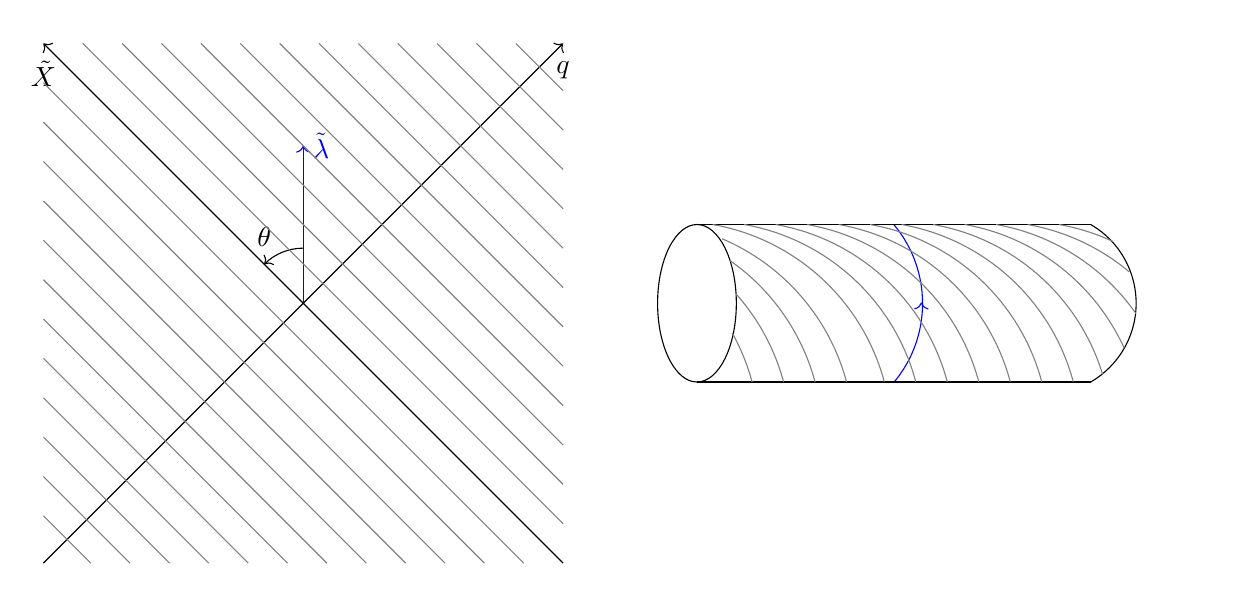
\begin{tikzpicture}
\clip (-3.5,-3.5) rectangle (11.5,3.5);

% \draw[color=gray,step=1.0,dotted] (-3.3,-3.3) grid (3.3,3.3);

\draw[->] (-3.3,-3.3)--(3.3,3.3) node[below=3pt]{$q$};
\draw[->] (3.3,-3.3)--(-3.3,3.3) node[below=3pt]{$\tilde{X}$};
\draw[->,color=blue] (0,0)--(0,2) node[right]{$\tilde{\lambda}$};

\draw[->] (0,0.7) arc (90:135:0.7) node[above=3pt]{$\theta$};

\foreach \x in {1,...,12}
    \draw[color=gray, thin] (-3.3, 3.3-0.5*\x) -- (3.3-0.5*\x, -3.3);
\foreach \x in {1,...,12}
    \draw[color=gray, thin] (-3.3+0.5*\x, 3.3) -- (3.3, -3.3+0.5*\x);

\draw (5,0) ellipse (0.5 and 1);
\draw[->,color=blue] (7.85,0)--(7.85,0.01);
\draw[color=blue] (7.5,1) arc (40:-40:1.56);
\draw (10,1) arc (60:-60:1.1547);
\draw (5,1) -- (10,1);
\draw (5,-1) -- (10,-1);


\draw[color=gray, thin] (6.9,-1) arc (15:67:2.75);
\draw[color=gray, thin] (6.5,-1) arc (15:55:2.75);
\draw[color=gray, thin] (6.1,-1) arc (15:42:2.75);
\draw[color=gray, thin] (5.7,-1) arc (15:29:2.75);
\foreach \x in {0,...,6}
\draw[color=gray, thin] (5.2+0.4*\x,1) arc (80:15:2.75);
\draw[color=gray, thin] (8,1) arc (80:17:2.75);
\draw[color=gray, thin] (8.4,1) arc (80:24.5:2.75);
\draw[color=gray, thin] (8.8,1) arc (80:35:2.75);
\draw[color=gray, thin] (9.2,1) arc (80:50:2.75);
\draw[color=gray, thin] (9.6,1) arc (80:65:2.75);

% \fill (2.6,2.3) circle (0.05) node[left,color=blue]{$0$} node[right,color=black]{$z_0$};
% \fill (-2.6,2.4) circle (0.05) node[left, color=blue]{$\infty$} node[right,color=black]{$-\bar{z}_0$};
%
% \fill (0,2) circle (0.05) node[left]{$f(1)$};
% \fill (0,-2.4) circle (0.05) node[left]{$f(-1)$};
%
% \fill (0,0) circle (0.05) node[above=5pt, right, color=blue]{$\mu$} node[below=8.5pt, left,color=black]{$0$};
% \fill (1,0) circle (0.05) node[above, color=blue]{$\alpha$} node[below=1.7pt,color=black]{$1$};
% \fill (2.1,0) circle (0.05) node[above, color=blue]{$\beta$} node[below,color=black]{$k^{-1}$};
% \fill (-1,0) circle (0.05) node[above, color=blue]{$\bar{\alpha}^{-1}$} node[below=1.7pt,color=black]{$-1$};
% \fill (-2.1,0) circle (0.05) node[above, color=blue]{$\bar{\beta}^{-1}$} node[below,color=black]{$-k^{-1}$};

\end{tikzpicture}
\end{document}
